\documentclass[a4paper,english,12pt]{report}
%

\usepackage{amsmath}
\usepackage{amsfonts}
\usepackage{epsfig}
\usepackage{multicol}
\usepackage{wrapfig}
\usepackage{enumerate}
\usepackage{enumitem}
\usepackage[utf8]{inputenc}

\usepackage{geometry}

\geometry{
a4paper,
total={210mm,297mm},
left=20mm,
right=20mm,
top=20mm,
bottom=20mm,
bindingoffset=0mm
}

\newcommand{\meshup}[0]{\textsc{MeshUp}}
\newcommand{\cmake}[0]{\textsc{CMake}}
\newcommand{\rbdl}[0]{\textsc{RBDL}}
\newcommand{\muscod}[0]{\textsc{MUSCOD-II}}

%\def \Tfree {T^{\textup{free}}}
\def \Tfree {t^f}
\def \st {\textit{subject to:}}

\begin{document}
\thispagestyle{empty}

%%%%%%%%%%%%%%%%%%%%%%%%%%%%%%%%%%%%%%%%%%%%%%%%%%%%%%%%%%%%%%%%%%%%%%%%%

\section*{\muscod{}: Example 1: Rocket Car} 



Daniel Leineweber et al.

\begin{wrapfigure}{r}{0.35\textwidth}
	\begin{center}
		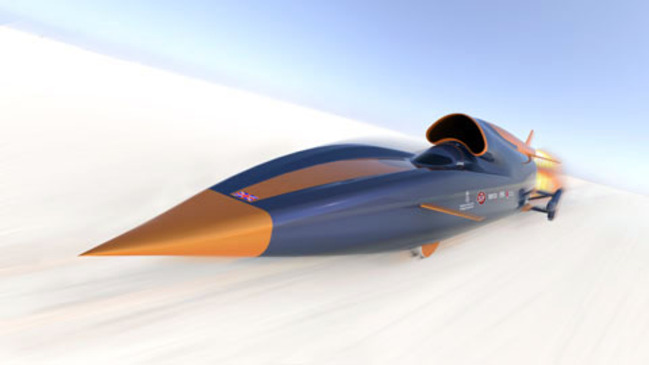
\includegraphics[width=0.3\textwidth]{rocketcar}
	\end{center}
	\caption{Rocket Car}
	\label{fig:rocketcar}
\end{wrapfigure}

\bigskip
\bigskip

This is a simple example that should get you started with MUSCOD. It is devoted to the introduction to one-phase optimal control problems. To this end we consider a rocket car, see Figure \ref{fig:rocketcar}.

\begin{itemize}
 \item The rocket car should drive for $300$m.
 \item The initial velocity at $t_0 = 0$ is $0$m/s. 
 \item The car can accelerate and brake between $-2$m/s$^2$ and $1$m/s$^2$.
 \item The maximum velocity is limited to $30$m/s.
 \item At final time $t_f$ the car should come to a complete stop. 
\end{itemize}


 
\subsection*{Tasks}

\begin{enumerate}
	\item Optimization 1: The car should drive for $32$s and then come to a complete stop. Minimize energy consumption.
	\item Optimization 2: Minimize final time.
\end{enumerate}
\medskip

\end{document}
